\documentclass{IOS-Book-Article}
\usepackage[utf8]{inputenc}
\usepackage{graphicx}

\def\hb{\hbox to 11.5 cm{}}

\newcommand{\sembrack}[1]{[\![#1]\!]}
\newcommand{\subex}[2]{#1_{#2}}
\newcommand{\commentOut}[1]{}
\newcommand{\eop}[1]{\mbox{\textsl{#1}}}
\newcommand{\ttop}[1]{\mbox{\texttt{#1}}}

\newcommand{\bequ}{\begin{quote}}
\newcommand{\enqu}{\end{quote}}
\newcommand{\bece}{\begin{center}}
\newcommand{\ence}{\end{center}}

\newenvironment{compactitem}{\begin{itemize}}{\end{itemize}}

\begin{document}

\pagestyle{headings}
\def\thepage{}
\begin{frontmatter}              % The preamble begins here.

\title{An End-to-End Pipeline from Law Text to Logical Formulas}

\markboth{}{August 2022\hb}

\author[A]{Aarne Ranta}
\author[B]{Inari Listenmaa}
\author[C]{Jerrold Soh}
\author[D]{Meng Weng Wong}

\address[A]{
  Department of Computer Science and Engineering,
  Chalmers University of Technology and University of Gothenburg,
  aarne.ranta@cse.gu.se 
  }
\address[B]{SMU and Digital Grammars}
\address[C]{SMU}
\address[D]{SMU}

\begin{abstract}
This paper describes an experimental pipeline starting from ordinary English law text, parsing it with a formal grammar, and converting it to logical formulas via a series of structural representations.
The goal is to see how to cover the full pipeline with a sequence of well-understood rule-based steps.
The approach is outside-in: we wanted to deliver some output from day 1, and refined it as we went on.
Thus it is a rule-based robust approach.
%%
The law text addressed is one chapter of law of Singapore, Part 6A of the Personal Data Protection Act 2012.
While more work is needed to port the method to other law texts, we believe to have achieved a reusable modular structure, as well as some reusable code, for a more general pipeline.
The pipeline includes some new methods and concepts, in particular, annotation-based grammar writing and an assemply logic for two-dimensional spreadsheet representations.
The code is available as open source.
\end{abstract}


\begin{keyword}
parsing law text
\end{keyword}
\end{frontmatter}
\markboth{August 2022\hb}{August 2022\hb}

%\maketitle




\section{Introduction}

Computational Law is an attempt to represent laws as computer programs.
Such programs can be used in expert systems, whose users can find out "what the law says" in different situations by posing explicit, concrete questions.
Some such systems are already in use, without even being called with that name.
For example, under the Covid-19 pandemic, travellers entering Singapore had to fill out web questionnaires about their country of origin, travel dates, and health data, and got an automatic answer telling them if they are allowed to enter and what test and quarantine plans they had to follow.

Setting up the Covid immigration system was a response to an emergency situation, where it would save work as possibly millions of people would be interested in entering the country, and their requests had to be treated efficiently.
The rules were, moreover, quite straightforward and unambiguous even if complex, and created in a time when web-based services were a normal way to organize things.
The situation is very different when it comes to laws in general: they may have a tradition of hundreds of years, so that decisions must be made by combining rules from different documents, which may seemingly contradict each othet and often be ambiguous.
Lawyers are needed to interpret them for laymen, case by case.
Lawyers are naturally also needed if laws are to be converted to expert systems.

The CCLAW project at Singapore Management University (SMU), School of Law, aims to develop technology that enables all laws of Singapore to be converted into computer systems.
The project uses natural language processing and theorem proving techniques, in particular, computational grammars and symbolic logics.
Many of the techniques are based on earlier work in computational law, but the ambition is somewhat different and more practical than in many other projects.
Thus the goal is to deal with the law as a whole, rather than selected and re-engineered fragments tailored to fit given methods.
The technology is also intended to leave room for a human in the loop: whenever the automated methods fail to give an unambiguous answer, a human lawyer can easily help it to take the decisive steps.
At the same time, the input required from the lawyer is reduced to the minimum, so that the routine coding work is carried out by the system.

From the technology point of view, CCLAW is building a classical pipeline where a parser converts a text to a formal representation, which is then converted to a set of logical formulas, for which an inference system exists or is developed.
In addition to the traditional components (syntax trees and logical formulas), the pipeline contains an intermediate spreadsheet representation of texts.
The spreadsheets aim to make the structure of the text explicit in a way that is readily accessible to lawyers, unlike syntax trees and formulas, which require training in formal logic and language theory.

The starting point of the project presented in this paper was a system consisting of \textbf{spreadsheets} and their translation to logical formulas.
The cells of the spreasheet were natural language expressions, which were parsed into syntax trees with the help of a grammar.
What was missing from the complete pipeline from text to logic was the conversion from the original text to spreadsheets.
This step was made manually, and the focus of the projects was on the later parts of the pipeline.
Thus the main contribution of the present paper is to define an automated conversion of texts to spreadsheets.
The first part of this is a grammar that parses texts to abstract syntax trees.
The second part is a conversion to a new intermediate representation between syntax trees, spreadsheets, and logic.
We call this representation \textbf{assembly logic}, in analogy to assembly languages in compilers, if we think of spreadsheets and logics as "machine languages", whose long distance to the source language is bridged by the assembly language.

Figure~\ref{pipeline} shows the complete pipeline.
\begin{figure}
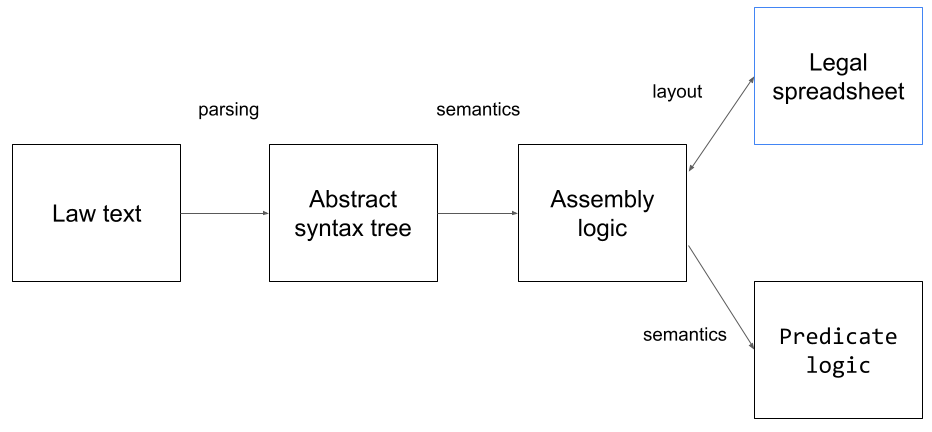
\includegraphics[width=0.8\textwidth]{pipeline.png}
\caption{The pipeline.}
\label{pipeline}
\end{figure}


\section{Building and using the grammar}


\section{Assembly logic and spreadsheets}


\section{Interpretation in predicate logic}


\section{Results, evaluation, and future work}


\section{Conclusion}


\begin{thebibliography}{99}


\bibitem{r1}
Petitti DB, Crooks VC, Buckwalter JG, Chiu V. Blood pressure levels before dementia.
Arch Neurol. 2005 Jan;62(1):112-6, doi: ....

\end{thebibliography}


\end{document}
